\documentclass[man]{apa6}
\usepackage{lmodern}
\usepackage{amssymb,amsmath}
\usepackage{ifxetex,ifluatex}
\usepackage{fixltx2e} % provides \textsubscript
\ifnum 0\ifxetex 1\fi\ifluatex 1\fi=0 % if pdftex
  \usepackage[T1]{fontenc}
  \usepackage[utf8]{inputenc}
\else % if luatex or xelatex
  \ifxetex
    \usepackage{mathspec}
  \else
    \usepackage{fontspec}
  \fi
  \defaultfontfeatures{Ligatures=TeX,Scale=MatchLowercase}
\fi
% use upquote if available, for straight quotes in verbatim environments
\IfFileExists{upquote.sty}{\usepackage{upquote}}{}
% use microtype if available
\IfFileExists{microtype.sty}{%
\usepackage{microtype}
\UseMicrotypeSet[protrusion]{basicmath} % disable protrusion for tt fonts
}{}
\usepackage{hyperref}
\hypersetup{unicode=true,
            pdftitle={The Sound of Intellect: Speech Reveals a Thoughtful Mind, Increasing a Job Candidate's Appeal},
            pdfauthor={Kamal Abdelrahman},
            pdfkeywords={keywords},
            pdfborder={0 0 0},
            breaklinks=true}
\urlstyle{same}  % don't use monospace font for urls
\usepackage{graphicx,grffile}
\makeatletter
\def\maxwidth{\ifdim\Gin@nat@width>\linewidth\linewidth\else\Gin@nat@width\fi}
\def\maxheight{\ifdim\Gin@nat@height>\textheight\textheight\else\Gin@nat@height\fi}
\makeatother
% Scale images if necessary, so that they will not overflow the page
% margins by default, and it is still possible to overwrite the defaults
% using explicit options in \includegraphics[width, height, ...]{}
\setkeys{Gin}{width=\maxwidth,height=\maxheight,keepaspectratio}
\IfFileExists{parskip.sty}{%
\usepackage{parskip}
}{% else
\setlength{\parindent}{0pt}
\setlength{\parskip}{6pt plus 2pt minus 1pt}
}
\setlength{\emergencystretch}{3em}  % prevent overfull lines
\providecommand{\tightlist}{%
  \setlength{\itemsep}{0pt}\setlength{\parskip}{0pt}}
\setcounter{secnumdepth}{0}
% Redefines (sub)paragraphs to behave more like sections
\ifx\paragraph\undefined\else
\let\oldparagraph\paragraph
\renewcommand{\paragraph}[1]{\oldparagraph{#1}\mbox{}}
\fi
\ifx\subparagraph\undefined\else
\let\oldsubparagraph\subparagraph
\renewcommand{\subparagraph}[1]{\oldsubparagraph{#1}\mbox{}}
\fi

%%% Use protect on footnotes to avoid problems with footnotes in titles
\let\rmarkdownfootnote\footnote%
\def\footnote{\protect\rmarkdownfootnote}


  \title{The Sound of Intellect: Speech Reveals a Thoughtful Mind, Increasing a Job Candidate's Appeal}
    \author{Kamal Abdelrahman\textsuperscript{1}}
    \date{}
  
\shorttitle{Speech Increases a Job Candidate’s Appeal}
\affiliation{
\vspace{0.5cm}
\textsuperscript{1} City University of New York - Brooklyn College}
\keywords{keywords\newline\indent Word count: X}
\usepackage{csquotes}
\usepackage{upgreek}
\captionsetup{font=singlespacing,justification=justified}

\usepackage{longtable}
\usepackage{lscape}
\usepackage{multirow}
\usepackage{tabularx}
\usepackage[flushleft]{threeparttable}
\usepackage{threeparttablex}

\newenvironment{lltable}{\begin{landscape}\begin{center}\begin{ThreePartTable}}{\end{ThreePartTable}\end{center}\end{landscape}}

\makeatletter
\newcommand\LastLTentrywidth{1em}
\newlength\longtablewidth
\setlength{\longtablewidth}{1in}
\newcommand{\getlongtablewidth}{\begingroup \ifcsname LT@\roman{LT@tables}\endcsname \global\longtablewidth=0pt \renewcommand{\LT@entry}[2]{\global\advance\longtablewidth by ##2\relax\gdef\LastLTentrywidth{##2}}\@nameuse{LT@\roman{LT@tables}} \fi \endgroup}


\DeclareDelayedFloatFlavor{ThreePartTable}{table}
\DeclareDelayedFloatFlavor{lltable}{table}
\DeclareDelayedFloatFlavor*{longtable}{table}
\makeatletter
\renewcommand{\efloat@iwrite}[1]{\immediate\expandafter\protected@write\csname efloat@post#1\endcsname{}}
\makeatother

\authornote{Kamal Abdelrahman is an undergraduate at the City University of New York - Brooklyn College in Brooklyn, NY majoring in psychology with a focus in statistical programming.

Correspondence concerning this article should be addressed to Kamal Abdelrahman, Brooklyn, NY. E-mail: \href{mailto:kamalabdel97@gmail.com}{\nolinkurl{kamalabdel97@gmail.com}}}

\abstract{
This study is an exact replication of Juliana Schroeder \& Nicholas Epley's (2015) experiment of whether a potential job candidate is percieved more intelligent through text or audio. 39 Forturne 500 company recruiters rated job candidates on their intellect, a composite score of the candidate's intelligence, competence, and thoughtfulness. They hypothesized that speech communicates intelligence better than written words. This study recreated the analysis of regarding presenation of pitches and their favorability. Analysis supported that hypothesis.


}

\begin{document}
\maketitle

\hypertarget{introduction}{%
\section{Introduction}\label{introduction}}

An interview is a key moment in every job applicant's hiring process, as it provides the opportunity for the hiring manager and the interviewee to discuss a potential match within the company. For the interviewer, it's about picking the right candidate. For the interviewee, it's about picking the right style of presentation. Schroeder \& Epley (2015) bring this into question with their study, in which they investigate the effects of audio and written presentations in an interview.

\hypertarget{methods}{%
\section{Methods}\label{methods}}

\emph{Participants}

In this study, there were 39 participants, all professional Fortune 500 recruiters. The average of age the recruiters was \emph{M} = 30.85 (\emph{SD} = 6.24). 10.3\% of the participants are male and 76.9\% are female.

\emph{Materials}

Two materials were used in this analysis. The first material was the dataset used in Schroeder \& Epley's study from githhub. The dataset could be accessed \href{\%22https://raw.githubusercontent.com/CrumpLab/statisticsLab/master/data/SchroederEpley2015data.csv\%22}{here} The data was analyzed so that the t-test could be reproduced.

The second material was R Studio, the Integrated Development Environemnt (IDE) for R. The IDE was used as a platform to analyze the dataset in R.

\newpage

\emph{Procedure}

To recreate this analysis of the t-test the data was loaded into R from \href{\%22https://raw.githubusercontent.com/CrumpLab/statisticsLab/master/data/SchroederEpley2015data.csv\%22}{Github} with the \emph{fread} function of the data.table library (Dowle \& Srinivasan, 2018).

\hypertarget{results}{%
\section{Results}\label{results}}

An independent samples t-test was conducted to examine the manipulation effects of audio and written expressions of intelligence in potential employees. Interviewees who expressed their intelligence through spokem during their interviews were rated significantly better (\emph{M} = 6.43, \emph{SD} = 1.43) than interviewees who wrote out their responses (\emph{M} = 4.39, \emph{SD} = 2.17) \(t(37) = -3.53\), \(p = .001\), \(d_{s}\) = -1.13

\begin{figure}
\centering
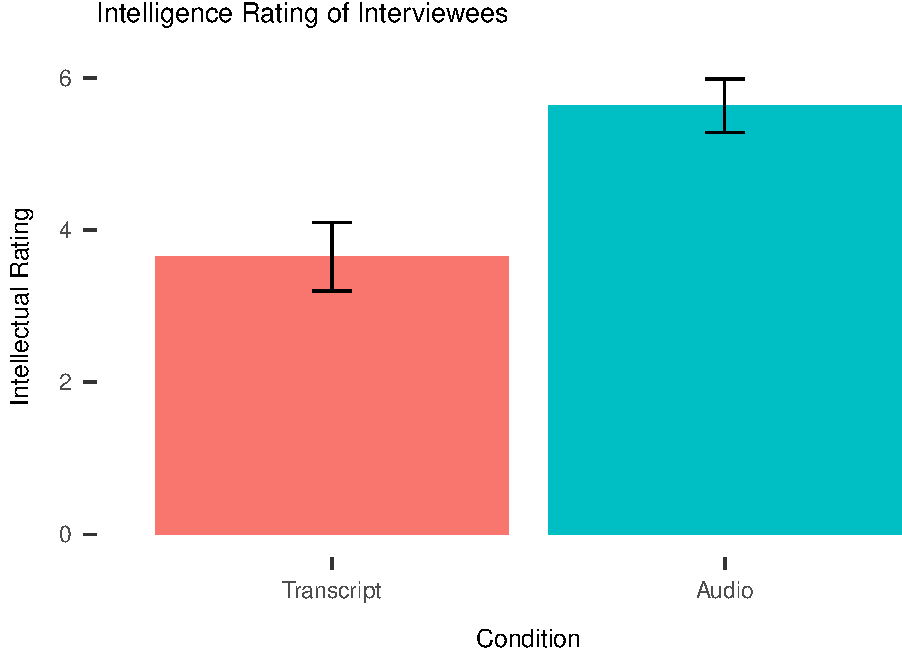
\includegraphics{SchroederEpley2015_files/figure-latex/f1-1.pdf}
\caption{\label{fig:f1}THE}
\end{figure}

\begin{table}[tbp]
\begin{center}
\begin{threeparttable}
\caption{\label{tab:rt}Descriptive statistics of intellectual ratings by presentation method.}
\begin{tabular}{lll}
\toprule
CONDITION & \multicolumn{1}{c}{Mean} & \multicolumn{1}{c}{SD}\\
\midrule
Transcript & 4.65 & 1.91\\
Audio & 6.63 & 1.61\\
\bottomrule
\end{tabular}
\end{threeparttable}
\end{center}
\end{table}

\hypertarget{discussion}{%
\section{Discussion}\label{discussion}}

Schroeder and Epley hypothesized that a person is a more appealing job candidate if they communicated with their voice as opposed to with text. Results supported this hypothesis, which stated that candidates who communicated through audio were rated significantly more desirable than canidates who did not. This analysis was consistent across all five experiments that were conducted. This aligns well with other studies which have focused on speech style, particuarly that interviewees who spoke more powerfully were rated positively for competence and employability (Parton, Siltanen, Hosman, \& Langenderfer, 2002) This study could further build on their findings to identify the effects of tone pitch on likeability.

\hypertarget{simulation}{%
\section{Simulation}\label{simulation}}

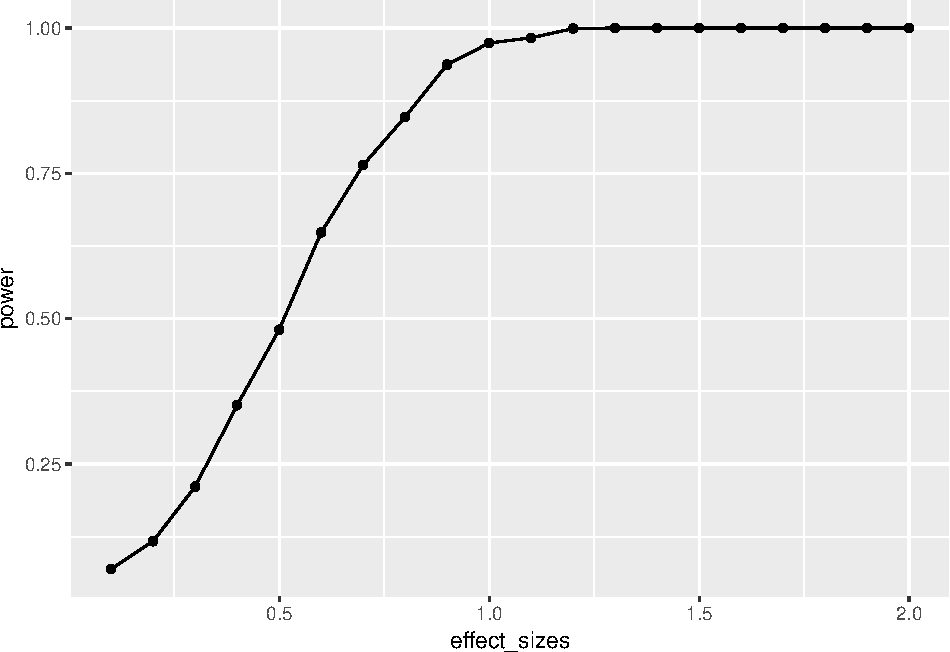
\includegraphics{SchroederEpley2015_files/figure-latex/unnamed-chunk-4-1.pdf}

```

\newpage

\hypertarget{references}{%
\section{References}\label{references}}

\begingroup
\setlength{\parindent}{-0.5in}
\setlength{\leftskip}{0.5in}

\hypertarget{refs}{}
\leavevmode\hypertarget{ref-R-data.table}{}%
Dowle, M., \& Srinivasan, A. (2018). \emph{Data.table: Extension of `data.frame`}. Retrieved from \url{https://CRAN.R-project.org/package=data.table}

\leavevmode\hypertarget{ref-parton2002employment}{}%
Parton, S. R., Siltanen, S. A., Hosman, L. A., \& Langenderfer, J. (2002). Employment interview outcomes and speech style effects. \emph{Journal of Language and Social Psychology}, \emph{21}(2), 144--161.

\leavevmode\hypertarget{ref-schroeder2015sound}{}%
Schroeder, J., \& Epley, N. (2015). The sound of intellect: Speech reveals a thoughtful mind, increasing a job candidate's appeal. \emph{Psychological Science}, \emph{26}(6), 877--891.

\endgroup


\end{document}
